%!TEX root = ../PTC-LibUG.tex

\chapter{Data Types}

\index{data types!described}
This appendix contains descriptions and examples of the \Fninety\ data that \PTC\ uses for $s$-based tracking and time-based tracking.

\fxnote{Al: I copied the TYPE definitions is this appendix from the ptc_2008_8_14 folder. I copied the definitions verbatim with two exceptions: I corrected obvious typos such as PONITER, and I retyped lowercase as uppercase.}


\section{S-based Tracking}

\index{s-based tracking!data types}
This section discusses the following \PTC\ data types for $s$-based tracking
and gives the \Fninety\ definitions for several important types:
\begin{itemize}
  \item layout,
  \item fibre,
  \item chart, including magnet frame,
  \item patch.
\end{itemize}


\subsection{Layout}

\index{layout!defined}
\index{data type!\ptc{LAYOUT}}
\index{LAYOUT@\ptc{LAYOUT}!data type}
\index{linked list!layout}
The \ptc{LAYOUT} type is a doubly linked list whose nodes, of data type
\ptc{FIBRE}, contain the magnet, the local charts, and the patches.

\begin{ptccode}
TYPE LAYOUT
  CHARACTER(120), POINTER ::\  NAME  ! IDENTIFICATION
  INTEGER, POINTER ::\  INDEX,HARMONIC_NUMBER  ! IDENTIFICATION, CHARGE SIGN
  LOGICAL(LP),POINTER ::\ CLOSED
  INTEGER,  POINTER ::\ N  ! TOTAL ELEMENT IN THE CHAIN
  INTEGER,POINTER ::\ NTHIN
  ! NUMBER IF THIN LENSES IN COLLECTION  (FOR SPEED ESTIMATES)
  REAL(DP),  POINTER ::\ THIN
  ! PARAMETER USED FOR AUTOMATIC CUTTING INTO THIN LENS
  !\ POINTERS OF LINK LAYOUT
  INTEGER, POINTER ::\ LASTPOS  ! POSITION OF LAST VISITED
  TYPE (FIBRE), POINTER ::\ LAST  ! LAST VISITED
  !
  TYPE (FIBRE), POINTER ::\ END
  TYPE (FIBRE), POINTER ::\ START
  TYPE (FIBRE), POINTER ::\ START_GROUND
  ! STORE THE GROUNDED VALUE OF START DURING CIRCULAR SCANNING
  TYPE (FIBRE), POINTER ::\ END_GROUND
  ! STORE THE GROUNDED VALUE OF END DURING CIRCULAR SCANNING
  TYPE (LAYOUT), POINTER ::\ NEXT
  TYPE (LAYOUT), POINTER ::\ PREVIOUS
  TYPE(NODE_LAYOUT), POINTER ::\ T  !  ASSOCIATED  CHILD THIN LENS LAYOUT
  TYPE (MAD_UNIVERSE), POINTER ::\ PARENT_UNIVERSE
  TYPE(LAYOUT_ARRAY), POINTER ::\ DNA(:)
  !   TYPE(SIAMESE_ARRAY), POINTER ::\ GIRDER(:)
  !   TYPE(JUNCTION_ARRAY), POINTER ::\ CON2(:)
END TYPE LAYOUT
\end{ptccode}

The first lines of the \ptc{TYPE} definition contain data specific to the layout
itself: data concerning steps of integration statistics.

Besides the fibres, the two most important quantities in this layout are \ptc{N}
and \ptc{CLOSED}. The variable \ptc{N} is the number of fibres in the layout.
\ptc{N} is updated each time magnets are inserted or deleted. The boolean 
\ptc{CLOSED} refers to the topology of the so-called ``base space'' or, in
accelerator parlance, the $s$-variable. Is the variable $s$ periodic (a ring),
or is the variable $s$ defining an interval (a straight beam line)? In the case of
a ring, \ptc{CLOSED} is set to true, otherwise it is set to false. This does not
happen automatically: the user must set it to the desired value.

The pointer T points to the layout's its associated \ptc{NODE_LAYOUT}.
This pointer is normally grounded because \PTC\ does not systematically
create node layouts or \emph{thin layouts}. When not grounded, the pointer
contains the expanded representation displayed on the left side of
\fref{TYPE.INTEGRATION.NODE}.

\fxnote{Al: Am I correct that node layout and thin layout are synonyms? If not, the above description must be changed.}

\fref[c]{Layout-link-list-fibres} illustrates the roles of the pointer
variables. The figure shows a layout with four elements. Obviously, the
number of elements in an actual beam line could be enormous.

\begin{figure}[ht]\forcerectofloat
  \centering
  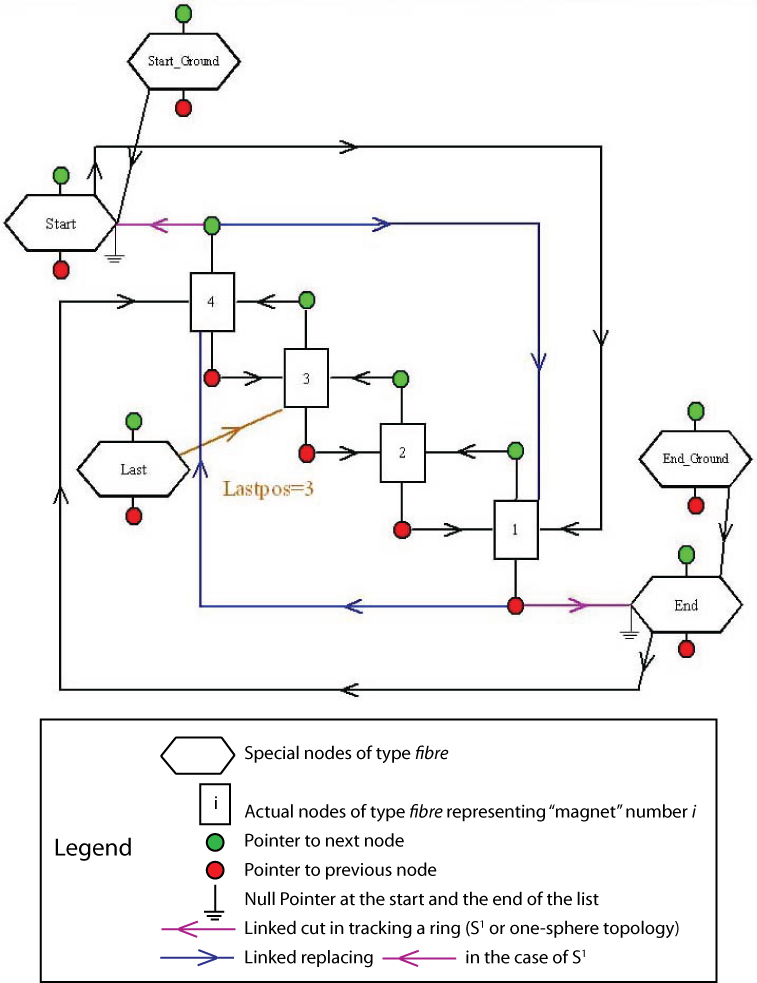
\includegraphics[width=.9\textwidth]{illustrations/fibre}
  \caption{A layout is a linked list of fibres.}
  \label{fig:Layout-link-list-fibres}
\end{figure}

First of all, a linked list must have at least one pointer; this allows
the creation of a simple linked list rather than a doubly linked list.
In our case this role is played by the pointer \ptc{PREVIOUS}. In
a simple linked list, each node has the red \ptc{PREVIOUS} pointer.
The pointer \ptc{END} points to the end of the list, in our case fibre 4.
Then the list is traversed backwards using the pointer \ptc{PREVIOUS}.

A more complex structure is required to handle two-way traversing.
To do this, we use the pointer \ptc{START}. At each node we add
the green pointer \ptc{NEXT}. The green pointer points to the next element
until it finally ends on the \ptc{START} pointer. The \ptc{START} pointer
as well as the \ptc{END} pointer are nullified or grounded. Thus one can
perform an ``ASSOCIATED'' check on either \ptc{NODE\%NEXT}
or \ptc{NODE\%PREVIOUS} to determine if the extremities of the list have
been reached.

We want to have a \emph{circular }linked list for tracking a ring. When
circular, the magenta link pointing to the grounded \ptc{START} is cut.
The last fibre's green pointer now points to fibre 1 (blue link). Thus the
list is made circular in the forward direction. The purpose of the 
\ptc{START GROUND} pointer is to remember the location of the grounded
\ptc{START} pointer to re-establish the ordinary two-way terminated list if
necessary. The same type of operation is performed on the magenta link
pointing to the \ptc{END} pointer. The list is the fully circular. \PTC\ routines
permit a programmer to toggle back and fourth between terminated and
circular lists.

The \ptc{LAST} pointer remembers the last fibre which was accessed by
any of the maintenance routines. This allows the routine \ptc{MOVE TO}, 
which locates an actual fibre, to find its target faster. In our case speed is
not of great importance. We tend to traverse a \ptc{LAYOUT} in the order
of tracking.


\subsection{Fibre}

\index{fibre!defined}
\index{data type!\ptc{FIBRE}}
\index{FIBRE@\ptc{FIBRE}!data type}
The type \ptc{FIBRE} is recursively defined. This allows the creation
of a linked list. One can think of a linked list as a chain; data potentially
hangs on each link. In our case, the fundamental datum is the object
\ptc{CHART} of data type \ptc{CHART}. This contains three actual charts
(affine frames of reference): one at each end of the fibre and one in the middle.

\begin{ptccode}
TYPE FIBRE
  !  BELOW ARE THE DATA CARRIED BY THE NODE
  INTEGER,POINTER ::DIR
  TYPE(PATCH),POINTER ::PATCH
  TYPE(CHART),POINTER ::CHART
  TYPE (ELEMENT), POINTER ::  MAG
  TYPE (ELEMENTP),POINTER ::  MAGP
  !  END OF DATA
  !  POINTER TO THE MAGNETS ON EACH SIDE OF THIS NODE
  TYPE (FIBRE),POINTER :: PREVIOUS
  TYPE (FIBRE),POINTER :: NEXT
  !  POINTING TO PARENT LAYOUT AND PARENT FIBRE DATA
  TYPE (LAYOUT),POINTER :: PARENT_LAYOUT
  TYPE(INFO),POINTER ::I
  TYPE(INTEGRATION_NODE),POINTER :: T1,T2
  ! FIRST AND LAST INTEGRATION_NODE CHILDREN CORRESPOUNDING TO PATCHES
  TYPE(INTEGRATION_NODE),POINTER :: TM  ! MIDDLE INTEGRATION_NODE
  INTEGER,POINTER ::POS     ! POSITION IN LAYOUT
  ! NEW STUFF....
  REAL(DP), POINTER :: BETA0,GAMMA0I,GAMBET,MASS  !,P0C
  INTEGER, POINTER :: CHARGE
  REAL(dDP), POINTER :: AG
  ! TO TIE LAYOUTS
  TYPE (FIBRE),POINTER :: P
  TYPE (FIBRE),POINTER :: N
  INTEGER,POINTER :: LOC
END TYPE FIBRE
\end{ptccode}

The type definition includes the beam element \ptc{MAG} and its polymorphic version
\ptc{MAGP}. \ptc{MAG} is the generic magnet to which we attach a single particle
propagator. \ptc{MAGP} is almost a carbon copy of \ptc{MAG}. The integer
\ptc{DIR} defines the direction of propagation through the fibre. We can
enter the magnet either from the front or from the back. \ptc{P0C} and
\ptc{BETA0} define a preferential frame of reference for the energy of this fibre.
It is usually the same as the energy of the element \ptc{MAG}.

\fxnote{Al: Is the above description of P0C and BETA0 correct? The text described an earlier version of the type definition. It looks like GAMMA0I, 
GAMBET, and MASS have replaced P0C.}

\ptc{T1} and \ptc{T2} are pointers to the first and last integration-node children.
The integer \ptc{POS} locates the fibre in the node layout. See
\fref{TYPE.INTEGRATION.NODE}.


\subsection{Chart}

\index{chart!defined}
\index{data type!\ptc{CHART}}
\index{CHART@\ptc{CHART}!data type}
Type \ptc{CHART} contains the information that locates an element in
three-dimensional space at the position where we want it to be.

\begin{ptccode}
TYPE CHART
  TYPE(MAGNET_FRAME), POINTER :: F
  !  FIBRE MISALIGNMENTS
  REAL(DP),DIMENSION(:),  POINTER::   D_IN,ANG_IN
  REAL(DP),DIMENSION(:),  POINTER::   D_OUT,ANG_OUT
END TYPE CHART
\end{ptccode}

\index{magnet frame!defined}
\index{data type!\ptc{MAGNET_FRAME}}
\index{MAGNET_FRAME@\ptc{MAGNET_FRAME}!data type}
\ptc{CHART} refers to the data type \ptc{MAGNET_FRAME}.

\begin{ptccode}
TYPE MAGNET_FRAME
  REAL(DP), POINTER,DIMENSION(:)  ::   A
  REAL(DP), POINTER,DIMENSION(:,:)::   ENT
  REAL(DP), POINTER,DIMENSION(:)  ::   O
  REAL(DP), POINTER,DIMENSION(:,:)::   MID
  REAL(DP), POINTER,DIMENSION(:)  ::   B
  REAL(DP), POINTER,DIMENSION(:,:)::   EXI
END TYPE MAGNET_FRAME
\end{ptccode}

\index{affine frame!attached to element}
\fref[c]{Charts-for-element} shows the three charts (affine frames of
reference) attached to an element.

\begin{figure}[ht]
  \centering
  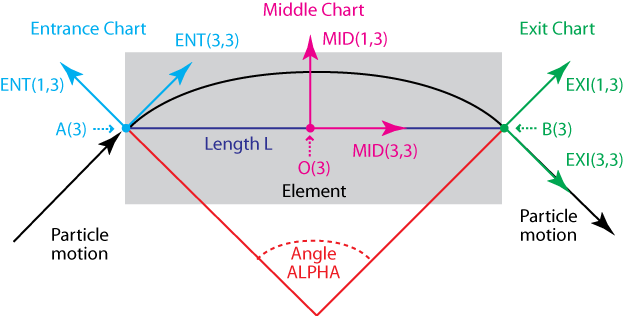
\includegraphics{illustrations/charts-for-element}
  \caption{Three charts attached to an element.}
  \label{fig:Charts-for-element}
\end{figure}

\fxnote{Al: Are MID(1,3) and MID(3,3) correct on the figure? My input figure shows them reversed, but it looks to me like MID(3,3) should follow the beam line.}

The variables \ptc{(A,ENT)}, \ptc{(O,MID)}, and \ptc{(B,EXI)} define the three charts. The variables \ptc{L} and \ptc{ALPHA} characterize the gray plane of the magnet. At the center of this plane lies the chart at $\Omega$. This is where a magnet is compressed for misalignment purposes.

The \ptc{TRACK} routine sends a ray from the cyan entrance chart
\ptc{(A,ENT)} through the middle chart \ptc{(O,MIS)} to the green exit
chart \ptc{(B,EXI)}.


\subsubsection{Misalignment}

\index{misalignment!contained in chart}
The \ptc{CHART} contains the misalignment information for a fibre (which,
of course, points to an element).

The variables \ptc{D_IN,ANG_IN} and \ptc{D_OUT,ANG_OUT} are
the displacements and rotations at the entrance and exit of the fibre.
In \fref{Misalignments-for-element}, the purple arrows represent
\ptc{D_IN} and \ptc{D_OUT}. The dotted purple arcs represent the angles
\ptc{ANG_IN} and \ptc{ANG_OUT}.

\begin{figure}[ht]\forceversofloat
  \centering
  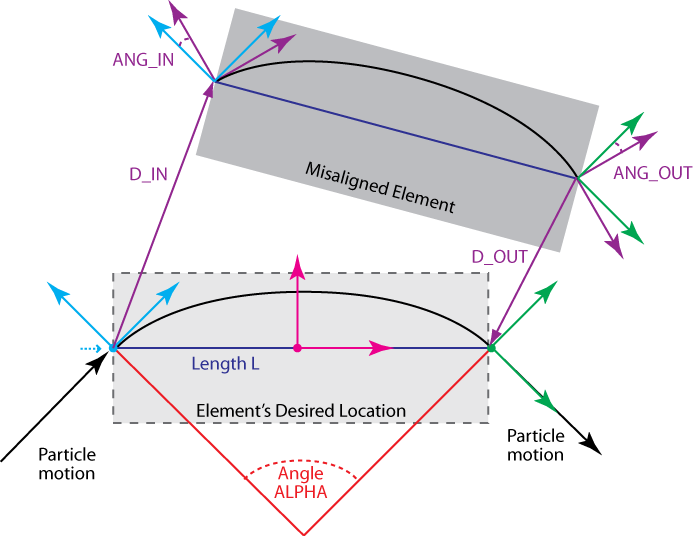
\includegraphics{illustrations/misalignment-for-element}
  \caption{Misalignments for a element.}
  \label{fig:Misalignments-for-element}
\end{figure}

\fref[c]{Misaligned-planar-fibre} provides a three-dimensional view
of a misaligned planar fibre. The position \ptc{FIBRE\%CHART\%F\%A(3)}
and the vector triad basis \ptc{FIBRE\%CHART\%F\%ENT(3,3)} specify the
fibre's desired location.

\begin{figure}[ht]
  \centering
  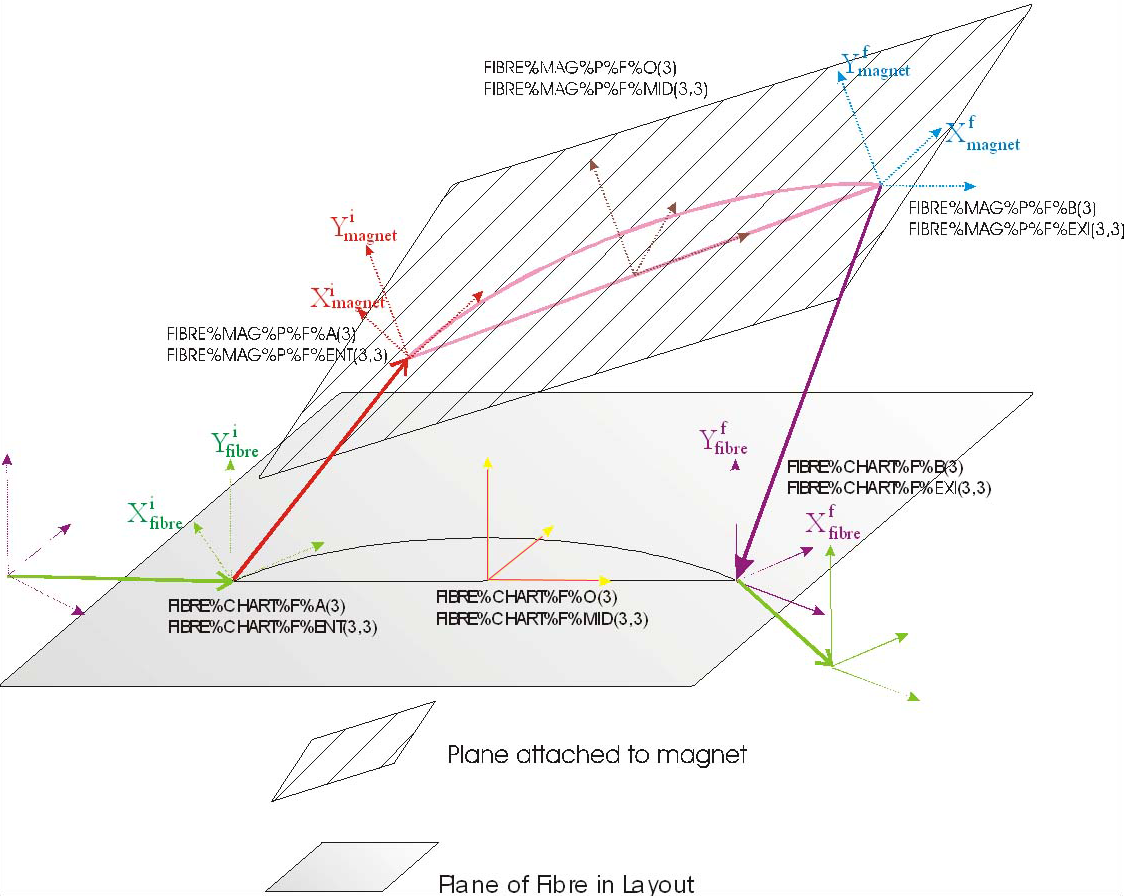
\includegraphics[width=\textwidth]{illustrations/misaligned-planar-fibre}
  \caption{Misaligned planar fibre in three dimensions.}
  \label{fig:Misaligned-planar-fibre}
\end{figure}


\subsection{Patch}

\index{patch!defined}
\index{data type!\ptc{PATCH}}
\index{PATCH@\ptc{PATCH}!data type}
The data type \ptc{PATCH} contains variables used in the main tracking loop to
perform certain adjustments if the exit chart of one element does
not connect smoothly with the entrance chart of the element that follows
it, for example, when transferring from one beam line to another.

\begin{ptccode}
TYPE PATCH
  INTEGER(2), POINTER:: PATCH
  ! IF TRUE, SPACIAL PATCHES NEEDED
  INTEGER, POINTER :: A_X1,A_X2
  ! FOR ROTATION OF PI AT ENTRANCE = -1, DEFAULT = 1 ,
  INTEGER, POINTER :: B_X1,B_X2
  ! FOR ROTATION OF PI AT EXIT = -1    , DEFAULT = 1
  REAL(DP),DIMENSION(:), POINTER:: A_D,B_D
  ! ENTRANCE AND EXIT TRANSLATIONS  A_D(3)
  REAL(DP),DIMENSION(:), POINTER:: A_ANG,B_ANG
  ! ENTRANCE AND EXIT ROTATIONS    A_ANG(3)
  INTEGER(2), POINTER:: ENERGY
  ! IF TRUE, ENERGY PATCHES NEEDED
  INTEGER(2), POINTER:: TIME
  ! IF TRUE, TIME PATCHES NEEDED
  REAL(DP), POINTER:: A_T,B_T
  ! TIME SHIFT NEEDED SOMETIMES WHEN RELATIVE TIME IS USED
END TYPE PATCH
\end{ptccode}


\section{Time-based Tracking}

\index{time-based tracking!data types}
This section discusses the following \PTC\ data types for time-based tracking
and gives the FORTRAN90 code:
\begin{itemize}
  \item integration node, including probe, temporal probe, and temporal beam,
  \item node layout, including beam.
\end{itemize}


\subsection{Integration Node}

\index{integration node!defined}
\index{data type!\ptc{INTEGRATION_NODE}}
\index{INTEGRATION_NODE@\ptc{INTEGRATION_NODE}!data type}
Integration nodes allow us to look at any point in the layout. One of
the most important applications is to permit collective forces. Moreover,
we can extend the coordinates of a particle to permit first-order
time-based tracking within the higher order $s$ framework. To do so,
we add to two coordinates to the particle:

\[
(\vec{z}=x,\, p_{x},\, y,\, p_{y},\, t,\, p_{t},\,\delta s,\, p_{n})\]

The coordinate $\delta s$ is the distance from the beginning
of the integration node measured in the coordinate $s$ used by the integrator.

The variable $p_n$ is a pointer to the integration node in which the particle
finds itself at time $t$.

During normal $s$-based tracking, $\delta s$ is always zero.
In a time-tracking mode, a drift is assumed between nodes to estimate the time
of a particle; the result $\delta s$ is computed. Since inverse drifts
are exactly known, this reduces to the normal $s$-based tracking when collective
effects are absent.

One immediate application is the tracking of several macro-particles in a recirculator
with important wake field effects between the macro-particles: time ordering of the
bunches is crucial and painlessly done in our framework.

\fxnote{Al: The above discussion may be more appropriate in Chapter 2's ``Modeling Particle Interactions''.}

The data type INTEGRATION_NODE is defined as follows:

\begin{ptccode}
TYPE INTEGRATION_NODE
  INTEGER, POINTER :: pos_in_fibre, CAS
  INTEGER, POINTER ::  pos
  real(dp), POINTER :: S(:)
  real(dp), POINTER :: ref(:)
  real(dp), pointer :: ent(:,:),a(:)
  real(dp), pointer :: exi(:,:),b(:)
  real(dp), POINTER :: delta_rad_in
  real(dp), POINTER :: delta_rad_out
  INTEGER, POINTER :: TEAPOT_LIKE
  TYPE (INTEGRATION_NODE), POINTER :: NEXT
  TYPE (INTEGRATION_NODE), POINTER :: PREVIOUS
  TYPE (NODE_LAYOUT), POINTER :: PARENT_NODE_LAYOUT
  TYPE(FIBRE), POINTER :: PARENT_FIBRE
  !   TYPE(EXTRA_WORK), POINTER :: WORK
  TYPE(BEAM_BEAM_NODE), POINTER :: BB
END TYPE INTEGRATION_NODE
\end{ptccode}

Each integration node is either

\begin{enumerate}
  \item the entrance patch/misalignment/tilt of its parent fibre (integration_node\%cas=-1);
  \item the entrance fringe field (integration_node\%cas=1);
  \item one of N steps in the body of the element (integration_node\%cas=0);
  \item the exit fringe field (integration_node\%cas=2);
  \item the exit patch/misalignment/tilt of its parent fibre (integration_node\%cas=-2).
\end{enumerate}

See \fref{TYPE.INTEGRATION.NODE}.

\begin{figure}[ht]\forcerectofloat
  \centering
  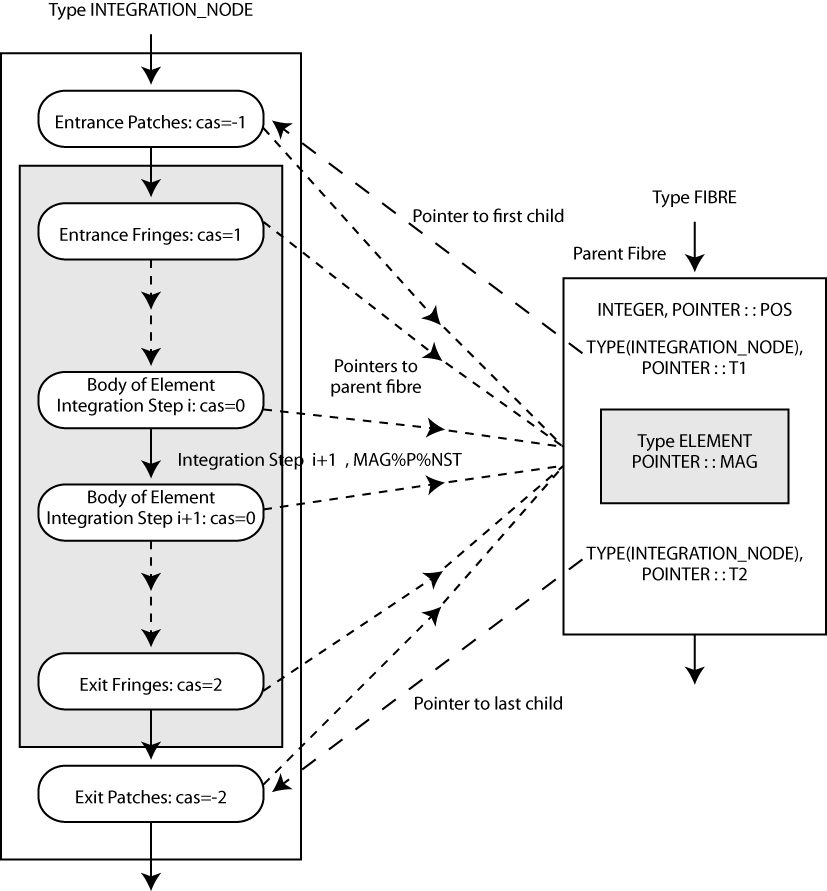
\includegraphics[width=\textwidth]{illustrations/integration-node-and-fibre}
  \caption{Type \ptc{integration_node} and type \ptc{fibre}.}
  \label{fig:TYPE.INTEGRATION.NODE}
\end{figure}

\ptc{NEXT} and \ptc{PREVIOUS} are the pointers necessary to create the \ptc{NODE_LAYOUT},
which is patterned closely on the \ptc{LAYOUT}.

\ptc{PARENT_FIBRE} points to the parent fibre which engendered the 
\ptc{INTEGRATION_NODE}.

\ptc{POS} is the position in the \ptc{NODE_LAYOUT}.

\ptc{POS_IN_FIBRE} is the position in the \ptc{PARENT_FIBRE}.

\ptc{TEAPOT_LIKE} indicates whether the internal frame of reference is
curved or straight. This is useful to move approximately inside an integration-node
step.

For \ptc{S}:
\begin{itemize}
  \item \ptc{S(1)} contains the ideal arc length position \ptc{LD},
  \item \ptc{S(2)} contains the local integration position \ptc{0<S(2)<L},
  \item \ptc{S(3)} contains the total \ptc{L} up to that integration node,%
  \footnote{This is similar to the survey L of MAD8 in the sense that for a
``real'' Cartesian bend the distance between the two parallel faces is used.
In other words, it is the sum around the ring of the integration variables,
whatever they may be. For a MAD-type RBEND it is still LD because these
bends are really sectors with wedges.}
  \item \ptc{S(4)} contains the length of the integration step 
  \ptc{DL : FIBRE\%MAG\%L/FIBRE\%MAG\%P\%NST}.
\end{itemize}


\subsubsection{Probe}
\label{sub:Probe-B}

\index{probe!defined}
\index{data type!\ptc{PROBE}}
\index{PROBE@\ptc{PROBE}!data type}
The data type \ptc{probe} holds information about the location of a particle.

\begin{ptccode}
TYPE PROBE
  REAL(DP) X(6)
  TYPE(SPINOR) S
  LOGICAL U
  TYPE(INTEGRATION_NODE),POINTER :: LOST_NODE
END TYPE PROBE
\end{ptccode}

The probe tracks position \ptc{X(6)} and spin \ptc{S}. The logical \ptc{U} is true if the particle is unstable.

\index{data type!\ptc{PROBE_8}}
\index{PROBE_8@\ptc{PROBE_8}!data type}
Here is the definition of the data type \ptc{PROBE_8}:

\begin{ptccode}
TYPE PROBE_8
  TYPE(REAL_8) X(6)
  TYPE(SPINOR_8) S
  REAL(DP) E_IJ(NDIM2,NDIM2)
  LOGICAL U
  TYPE(INTEGRATION_NODE),POINTER :: LOST_NODE
END TYPE PROBE_8
\end{ptccode}

\fxnote{Al: What does a PROBE_8 do? \'Etienne provided its
type definition with the material on Tracking Routines on Integration Nodes.}


\subsubsection{Temporal Probe}
\label{sub:Temporal-Probe-B}

\index{data type!\ptc{TEMPORAL_PROBE}}
\index{TEMPORAL_PROBE@\ptc{TEMPORAL_PROBE}!data type}
The data type \ptc{temporal probe }holds a probe and information relevant to 
time-based tracking.

\begin{ptccode}
TYPE TEMPORAL_PROBE
  TYPE(PROBE) XS
  TYPE(INTEGRATION_NODE), POINTER :: NODE
  REAL(DP) DS,POS(6)
  TYPE(INTERNAL_STATE) STATE
END TYPE TEMPORAL_PROBE
\end{ptccode}

The probe \ptc{XS} contains the coordinates.

The \ptc{NODE} points to the integration node that the particle is in.

The distance \ptc{DS} is the approximate distance that the particle
traveled inside the node, assuming a drift.

\ptc{POS(6)} is the position of the particle in an absolute 3D frame.

\ptc{STATE} is the tracking state of that beam/machine.

\fxnote{Al: I couldn't find a type definition for a temporal probe or a temporal beam in the inc files in the PTC_2008_8_14 folder. Did I miss those type definitions? (I couldn't find a type definition for a probe, either, but \'Etienne provided it in his Tracking Routines document.)}


\subsubsection{Temporal Beam}
\label{sub:Temporal-Beam-B}

\index{temporal beam!defined}
\index{data type!\ptc{TEMPORAL_BEAM}}
\index{TEMPORAL_BEAM@\ptc{TEMPORAL_BEAM}!data type}
The data type \ptc{temporal beam }is a collection of particles (probes).

\begin{ptccode}
TYPE TEMPORAL_BEAM
  TYPE(TEMPORAL_PROBE), POINTER :: TP(:)
  REAL(DP) A(3),ENT(3,3),P0C,TOTAL_TIME
  INTEGER N
  TYPE(INTEGRATION_NODE),POINTER :: C  ! POINTER CLOSE TO A(3)
  TYPE(INTERNAL_STATE) STATE
END TYPE TEMPORAL_BEAM
\end{ptccode}

A temporal beam must be allocated:

\begin{ptccode}
CALL ALLOC(TB,N,P0C)
\end{ptccode}

\ptc{P0C} is the reference momentum of the beam.

We must set the initial conditions of the layout:

\begin{ptccode}
CALL POSITION_TEMPORAL_BEAM(LAYOUT,TB,STATE)
\end{ptccode}

\index{routine!\ptc{POSITION_TEMPORAL_BEAM}}
\index{POSITION_TEMPORAL_BEAM@\ptc{POSITION_TEMPORAL_BEAM}!routine}
\index{routine!\ptc{LOCATE_TEMPORAL_BEAM}}
\index{LOCATE_TEMPORAL_BEAM@\ptc{LOCATE_TEMPORAL_BEAM}!routine}
\index{routine!\ptc{ORIGINAL_P_TO_PTC}}
\index{ORIGINAL_P_TO_PTC@\ptc{ORIGINAL_P_TO_PTC}!routine}
\index{momenta!adjusting}
%
The subroutine \ptc{POSITION_TEMPORAL_BEAM}
\begin{itemize}
  \item locates the beam in three dimensions and stores \ptc{TB\%TP(i)\%POS(1:3)=(X,Y,Z)},
  which is \PTC's global frame;
  \item calls the \ptc{LOCATE_TEMPORAL_BEAM} routine, which in turn calls the
   \ptc{ORIGINAL_P_TO_PTC} routine, which adjusts the momenta.
\end{itemize}

The beam's values of \ptc{TB\%TP(i)\%XS\%X(1:6)} are now in \PTC's local
coordinates.


\subsection{Node Layout}

\index{node layout!defined}
\index{data type!\ptc{NODE_LAYOUT}}
\index{NODE_LAYOUT@\ptc{NODE_LAYOUT}!data type}
\index{beam line!expanded}
\index{linked list!node layout}
%
The data type \ptc{NODE_LAYOUT} is a linked list of nodes,
which represents an expanded beam line. The nodes do not contain new
data; their fibres contain their data.

The type \ptc{NODE_LAYOUT} is defined as follows:

\begin{ptccode}
TYPE NODE_LAYOUT
  CHARACTER(120), POINTER ::  NAME ! IDENTIFICATION
  INTEGER, POINTER ::  INDEX ! IDENTIFICATION
  LOGICAL(LP),POINTER ::CLOSED
  INTEGER,  POINTER :: N  ! TOTAL ELEMENT IN THE CHAIN
  ! POINTERS OF LINK LAYOUT
  INTEGER, POINTER :: LASTPOS   ! POSITION OF LAST VISITED
  TYPE (INTEGRATION_NODE), POINTER :: LAST ! LAST VISITED
  !
  TYPE (INTEGRATION_NODE), POINTER :: END
  TYPE (INTEGRATION_NODE), POINTER :: START
  TYPE (INTEGRATION_NODE), POINTER :: START_GROUND
  ! STORE THE GROUNDED VALUE OF START DURING CIRCULAR SCANNING
  TYPE (INTEGRATION_NODE), POINTER :: END_GROUND
  ! STORE THE GROUNDED VALUE OF END DURING CIRCULAR SCANNING
  TYPE (LAYOUT), POINTER :: PARENT_LAYOUT
  TYPE(ORBIT_LATTICE), POINTER :: ORBIT_LATTICE
END TYPE NODE_LAYOUT
\end{ptccode}


\subsubsection{Beam}
\label{sub:Beam-B}

\index{data type!\ptc{BEAM}}
\index{BEAM@\ptc{BEAM}!data type}
The purpose of the node layout is to track a beam. We now define the
data type \ptc{BEAM}.

\begin{ptccode}
TYPE BEAM
  !   TYPE(REAL_8), POINTER :: Y(:)
  REAL(DP), POINTER :: X(:,:)
  !   REAL(DP), POINTER :: SIGMA(:),DX(:),BBPAR,ORBIT(:)
  LOGICAL(LP), POINTER :: U(:)
  TYPE(BEAM_LOCATION), POINTER::POS(:)
  INTEGER, POINTER :: N,LOST
  !   INTEGER, POINTER :: CHARGE
  !   LOGICAL(LP),POINTER :: TIME_INSTEAD_OF_S
  !   LOGICAL(LP),POINTER :: BEAM_BEAM,BBORBIT
END TYPE BEAM
\end{ptccode}

\index{data type!\ptc{BEAM_LOCATION}}
\index{BEAM_LOCATION@\ptc{BEAM_LOCATION}!data type}
We also define the data type \ptc{BEAM_LOCATION}:

\begin{ptccode}
TYPE BEAM_LOCATION
  TYPE (INTEGRATION_NODE), POINTER :: NODE
END TYPE BEAM_LOCATION
\end{ptccode}

\ptc{LOST} is the number of lost particles.

In a normal mode, the \ptc{BEAM} is pushed integration node to
integration node. It can also be pushed from a location \ptc{S1} to
\ptc{S2}.

\index{flag!\ptc{totalpath}}
\index{totalpath@\ptc{totalpath}!flag}
Additionally, time tracking is possible with \ptc{TOTALPATH=true}.
In that case, the position of the particle is given by specifying the
actual integration node immediately proceeding the particle and the 
distance from that integration node measured in the integration
variable \ptc{L}. The node is located using the pointer
\ptc{POS(:)\%Node}, and the distance is located in \ptc{X(:,:)}.
Drifting back and forth to that position is done approximately with
a drift either in Cartesian or Polar coordinates depending on the
variable \ptc{TEAPOT_LIKE} of the type \ptc{INTEGRATION_NODE}.


\fxnote{Al: I removed some text that I carried over from the \PTC\ website because the latest type definition for BEAM does not match the type definition on the website. I don't know how to update the comments to match the new type definition. The old type definition and text are below.}

\begin{ptccode}
TYPE BEAM
  REAL(DP), POINTER~:: X(N,1:7)
  LOGICAL(LP), POINTER :: U(N)
  TYPE(BEAM_LOCATION), POINTER::POS(N)
  INTEGER, POINTER :: N,LOST
  INTEGER, POINTER :: CHARGE
  LOGICAL(LP),POINTER :: TIME_INSTEAD_OF_S
END TYPE BEAM
\end{ptccode}

The array \ptc{X(N,1:7)} contains \ptc{N} (macro)particles whose \PTC\
co\"ordinates are located in \ptc{X(N,1:6)}. The array \ptc{U(N)} contains
a stability flag: true is unstable. \ptc{LOST} is the number of lost particles.

In the ``additionally'' paragraph, the third sentence originally read as follows:

``The node is located using the pointer \ptc{POS(N)\%Node} and the distance
is located in \ptc{X(N,7)}.''

\endinput
